\documentclass[doc, 12pt, donotrepeattitle]{apa6}
\usepackage[spanish]{babel}
\usepackage[utf8]{inputenc}
\usepackage{graphicx}
\graphicspath{ {img/} }

\title{Maratones de Programación
\\
Transformación y Normalización}
\shorttitle{Maratones de Programación --- Segunda Fase}
\author{Freddy Duran
\\
José Briceño
\\
Wilsen Hernandez}
\affiliation{Universidad de Carabobo
\\
Facultad Experimental de Ciencias y Tecnología
\\
Departamento de Computación
\\
Base de Datos}

\begin{document}
\maketitle
\section{Esquema Relacional}
\begin{itemize}
    \item \textbf{Equipo}(\underline{NombreEquipo}, AreaExpTecnico, Clasificacion, FechaCreacion, CargoCoach)
    \item \textbf{Integrante}(\underline{CI}, Nombre, Telefono, Direccion, Carrera, Tipo, FechaNac, NombreEquipo)
    
    \ \ \ \ c.f.: (NombreEquipo) referencia a \textbf{Equipo}.
    \item \textbf{Entrenamiento}(\underline{Tipo}, \underline{Fecha})
    \item \textbf{Competencia}(\underline{Region}, \underline{Fecha}, Sites, Nivel, Duracion, HoraInicio)
    \item \textbf{Problemas}(\underline{CodigoProblema}, Enunciado, Dificultad, TiempoLimiteSol, Region, Fecha)
    
    \ \ \ \ c.f.: (Region, Fecha) referencia a \textbf{Competencia}.
    \item \textbf{Reporte}(\underline{CI-Integrante}, \underline{Lugar}, \underline{Fecha}, Libros, Financia, Sitios, Otros)
    
    \ \ \ \ c.f.: (CI-Integrante) referencia a \textbf{Integrante}.
    \item \textbf{Incentivo-Integrante}(\underline{CI-Incentivado}, \underline{Incentivos})
    
    \ \ \ \ c.f.: (CI-Incentivado) referencia a \textbf{Integrante}.
    \item \textbf{Incidente-Viaje}(\underline{CI-Integrante}, \underline{Lugar}, \underline{Fecha}, Incidente)
    
    \ \ \ \ c.f.: (CI-Integrante) referencia a \textbf{Integrante}.
    
    \ \ \ \ c.f.: (Lugar, Fecha) referencia a \textbf{Reporte}.    
    \item \textbf{Recibe}(\underline{NombreEquipo}, \underline{Tipo}, \underline{Fecha})
    
    \ \ \ \ c.f.: (NombreEquipo) referencia a \textbf{Equipo}.
    
    \ \ \ \ c.f.: (Tipo, Fecha) referencia a \textbf{Entrenamiento}.
    \item \textbf{Participa}(\underline{NombreEquipo}, \underline{Region}, \underline{Fecha}, Ranking)
    
    \ \ \ \ c.f.: (NombreEquipo) referencia a \textbf{Equipo}.
    
    \ \ \ \ c.f.: (Region, Fecha) referencia a \textbf{Competencia}.
    \item \textbf{Resuelve}(\underline{NombreEquipo}, \underline{CodigoProblema}, Fecha, HoraEntrega, TipoSolucion, Lenguaje, TiempoSolucion)
    
    \ \ \ \ c.f.: (NombreEquipo) referencia a \textbf{Equipo}.
    
    \ \ \ \ c.f.: (CodigoProblema) referencia a \textbf{Problema}.
\end{itemize}

%\section{Normalización}
%\textbf{Equipo}(\underline{NombreEquipo}, AreaExpTecnico, Clasificacion, FechaCreacion, CargoCoach)

%\begin{center}
%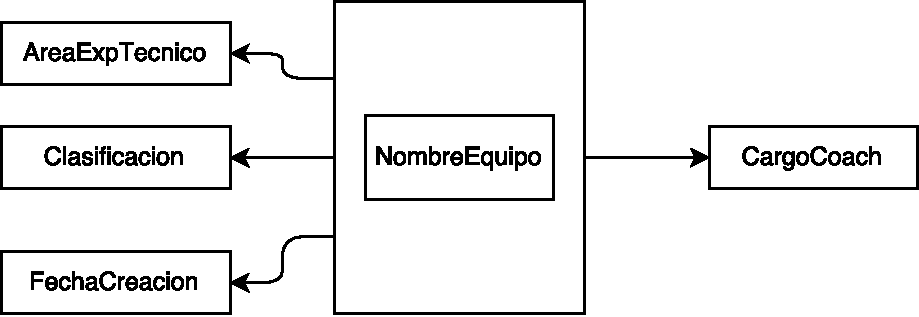
\includegraphics[scale=0.8]{NormalizacionEquipos}
%\end{center}

\end{document}
